\documentclass[a4paper,12pt]{article}
\title{Der Titel der Arbeit}
\author{Jon Doe}
% Umlaute im PDF sind nicht zusammengesetzt
\usepackage[T1]{fontenc}
% Umlaute müssen nicht maskiert werden
\usepackage[utf8]{inputenc}
% Vektorschriftart
\usepackage{lmodern}
% für Deutsche Begriffe und Silbentrennung
\usepackage[ngerman]{babel}
\usepackage{csquotes}
% Formeln
\usepackage{amsmath}
% Grafiken
\usepackage{graphicx}
% Abkürzungsverzeichnis
\usepackage[printonlyused]{acronym}
% Stichwortverzeichnis
\usepackage{makeidx}
\makeindex
% idxlayout works around a bug in LaTeX, which results in a wrong vertical position of the title
% http://tex.stackexchange.com/questions/23287/setting-the-same-distance-from-the-top-of-the-page-
% for-chapter-and-index-titles
\usepackage{idxlayout}
% Zeilenabstand 1,5 Zeilen
\usepackage{setspace}
\onehalfspacing
% BibLaTeX benutzen
\usepackage[backend=biber,citestyle=alphabetic,bibstyle=alphabetic]{biblatex}
\addbibresource{bib/Bibliographie.bib}
% Formatierung an Vorgaben anpassen
\DeclareLabelalphaTemplate{
	\labelelement{
		\field[final]{shorthand}
		\field{label}
		\field[strwidth=3,strside=left,ifnames=1]{labelname}
		\field[strwidth=1,strside=left]{labelname}
	}
	\labelelement{
	\literal{-}
	}
	\labelelement{
	\field[strwidth=2,strside=right]{year}
	}
}
% Seitenränder anpassen
\usepackage{geometry}
\geometry{left=2cm, right=2cm, top=2.5cm, bottom=2cm}
% eps-Grafiken
\usepackage{epstopdf}
% Siehe http://tex.stackexchange.com/questions/28198/using-ieeetrantools
\usepackage[retainorgcmds]{IEEEtrantools}

\usepackage{microtype}
\usepackage{blindtext}
\newcounter{savepage}
% pdf-Metadaten und Hyperlinks
\usepackage[pdfsubject = {{The subject of this thesis}},
			pdfkeywords = {{Keyword Keyword2}},
			pdfstartview = Fit,
			pdfpagelayout = SinglePage,
			hidelinks,
			pdfusetitle]{hyperref}
% Schneide automatisch alle mit /includegraphics eingebundene PDFs zu
\usepackage{xstring}
\let\oldincludegraphics\includegraphics
\renewcommand{\includegraphics}[2][width=\textwidth]{%
	\immediate\write18{pdfcrop #2}%
	\StrSubstitute{#2}{.pdf}{-crop.pdf}[\temp]%
	\oldincludegraphics[#1]{\temp}%
	}

\begin{document}
\pagenumbering{Roman}
\newpage\null\thispagestyle{empty}\newpage
\newpage
\pagestyle{empty}
\begin{figure}[t]
	\centering
	
\includegraphics[width=0.35\textwidth]{fig/Logo/h-da-logo-sw.pdf}
\end{figure}
\vfill
\begin{center}
\Large Hochschule Darmstadt \\
\normalsize \textsc{- Fachbereich Maschinenbau und Kunststofftechnik -} \\
\vfill
% \@title und \@author verfügbar machen
\makeatletter
\Huge \@title \\
\normalsize
\vspace{12pt}
Abschlussarbeit zur Erlangung des akademischen Grades \\
Bachelor of Science (B.Sc.)
\vfill
vorgelegt von \\
\@author
\makeatother
\vfill
\begin{tabular}[h]{p{4cm}l}
	Referent(in): & Name des Erstbetreuers\\
	Korreferent(in):  & Name des Zweitbetreuers \\
\end{tabular}
\end{center}
\newpage
\pagestyle{plain}
\section*{Eidesstattliche Erklärung}
\addcontentsline{toc}{section}{Eidesstattliche Erklärung}
Ich versichere hiermit, dass ich die vorliegende Arbeit selbständig verfasst und keine anderen als die im Literaturverzeichnis angegebenen Quellen benutzt habe. \\
\noindent Alle Stellen, die wörtlich oder sinngemäß aus veröffentlichten oder noch nicht veröffentlichten Quellen entnommen sind, sind als solche kenntlich gemacht. \\
\noindent Die Zeichnungen oder Abbildungen in dieser Arbeit sind von mir selbst erstellt worden oder mit einem entsprechenden Quellennachweis versehen. \\
\noindent Diese Arbeit ist in gleicher oder ähnlicher Form noch bei keiner anderen Prüfungsbehörde eingereicht worden.
\newline\newline
Darmstadt, den \today
\newpage
\phantomsection
\addcontentsline{toc}{section}{Abstract}
\let\oldabstractname\abstractname
\renewcommand{\abstractname}{Abstract}
\begin{abstract}
\blindtext \blindtext
\end{abstract}
\newpage
\phantomsection
\addcontentsline{toc}{section}{Zusammenfassung}
\let\abstractname\oldabstractname
\begin{abstract}
\blindtext \blindtext
\end{abstract}
\newpage
\section*{Vorwort}
\addcontentsline{toc}{section}{Vorwort}
\blindtext \blindtext
\newpage
\phantomsection
\addcontentsline{toc}{section}{Inhaltsverzeichnis}
\tableofcontents
% Letzte Seite mit römischer Seitenzahl speichern
\cleardoublepage
\setcounter{savepage}{\arabic{page}}
\newpage
\cleardoublepage
\pagenumbering{arabic}
% Struktur basiert auf http://kleinmann.eit.h-da.de/99_ThesisInfos/
\section{Einführung / Problembeschreibung}
Jemand "`musste"' Josef K. verleumdet haben, denn ohne dass er etwas Böses \cite{Pleisteiner.2007} getan hätte, wurde er eines Morgens verhaftet. »Wie ein Hund!« sagte er, es war, als sollte die Scham ihn überleben \ac{KDE} \cite[S.55ff]{Accardi.2010}. Als Gregor Sams eines Morgens aus unruhigen Träumen erwachte, fand er sich in seinem Bett zu einem ungeheuren Ungeziefer \index{Ungeziefer} verwandelt \cite{Lewis.2010}.
\subsection{Was ist die Motivation?}
\blindtext
Weiter unten im Text (S. 8) heißt es, dass es "`endgültige"' Leistungen in der Wissenschaft gar nicht geben könne.~\cite[S.~5--6]{Weber.1994b}
\begin{figure}[h]
	\centering 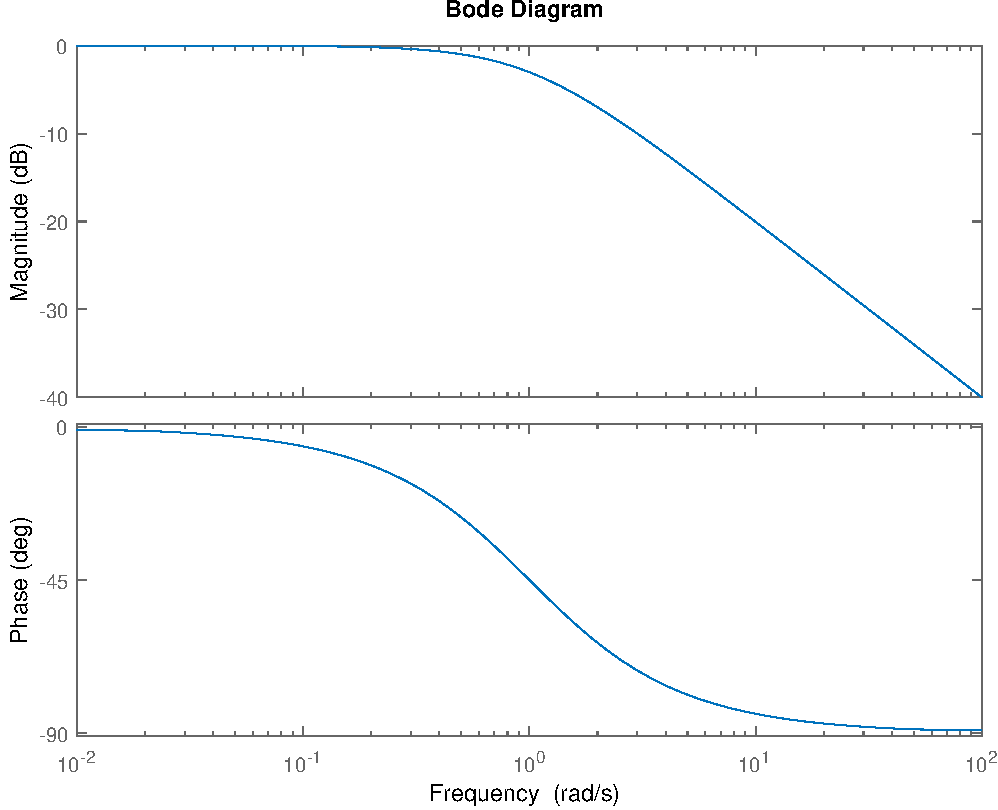
\includegraphics[width=0.5\textwidth]{fig/PT1/PT1-matlab.pdf}
	\caption{Bodediagramm PT1}
\end{figure}
\blindtext
\begin{IEEEeqnarray}{rCl}
	a & = & b + c \\
	& = & d + e + f + g + h \\
	& = & p + q + r + s
\end{IEEEeqnarray}
\blindtext
\begin{table}[h]
	\centering
	\begin{tabular}[h]{|c|c|}
		\hline
		$U_e$ / V& $U_a$ / V\\ \hline
		0.1 & 0.2 \\ \hline
		0.2 & 0.4 \\ \hline
		0.3 & 0.6 \\ \hline
		0.4 & 0.8 \\ \hline
		0.5 & 1 \\ \hline
	\end{tabular}
	\caption{Messergebnisse}
\end{table}
\subsection{Was ist die Aufgabe?}
\blindtext
\subsection{Was ist das Ziel dieser Arbeit?}
\blindtext
\subsection{Was war der Status Quo, bevor mit dieser Arbeit begonnen wurde?}
\blindtext
\subsubsection{Firma X hat etwas in der Vergangenheit auf diesem oder jenem Wege gemacht…}
\blindtext
\section{Problemlösung}
\blindtext
\subsection{Was sind die Optionen / Welche prinzipiellen Lösungen sind möglich?}
\blindtext
\subsection{Stand der Technik / Wie wird es woanders gemacht?}
\blindtext
\subsection{Was ist der in dieser Arbeit gewählte Ansatz?}
\blindtext
\subsection{Weshalb wurde dieser Ansatz gewählt / Was unterscheidet ihn von anderen / Was ist neu / Was ist bekannt?}
\blindtext
\subsection{Detaillierte Beschreibung der Problemlösung}
\blindtext
\section{Implementierung und Test}
\blindtext
\subsection{Wie wurde es implementiert}
\blindtext
\subsection{Wie wurde getestet}
\blindtext
\subsection{Warum wurde so getestet?}
\blindtext
\section{Validierung}
\blindtext
\subsection{Was sind die Ergebnisse}
\blindtext
\subsection{Vor- und Nachteile des entwickelten Systems}
\blindtext
\section{Zusammenfassung / Fazit / zukünftige Arbeit}
\blindtext
\subsection{Was wurde getan}
\blindtext
\subsection{Was muss noch getan werden / Wie kann das System verbessert werden?}
\blindtext
\newpage
\cleardoublepage
\pagenumbering{Roman}
% Seitenzahl wiederherstellen
\setcounter{page}{\thesavepage}
\clearpage
\phantomsection
\addcontentsline{toc}{section}{Literatur}
\printbibliography
\newpage
\renewcommand{\indexname}{Stichwortverzeichnis}
\printindex
\addcontentsline{toc}{section}{Stichwortverzeichnis}
\newpage
\section*{Abkürzungsverzeichnis}
\addcontentsline{toc}{section}{Abkürzungsverzeichnis}
\begin{acronym}[Bash] % längste Abkürzung
	\acro{KDE}{K Desktop Environment}
	\acro{SQL}{Structured Query Language}
	\acro{Bash}{Bourne-again shell}
	\acro{JDK}{Java Development Kit}
	\acro{VM}{Virtuelle Maschine}
	\acro{I2C}[IC]{Inter-Integrated Circuit}
\end{acronym}
\newpage
\phantomsection
\addcontentsline{toc}{section}{Abbildungsverzeichnis}
\listoffigures
\newpage
\phantomsection
\addcontentsline{toc}{section}{Tabellenverzeichnis}
\listoftables
\newpage
\section*{Anhang}
\addcontentsline{toc}{section}{Anhang}
\end{document}